\newpage
\section{Benchmarks}

Les benchmarks suivants ont été réalisés sur plafrim, les scripts d'obtention sont présents dans les sources et fonctionnent également sur des ordinateurs personnels. Nous nous sommes plus particulièrement intéressés aux \emph{speedups} : le temps que met l'implémentation étudiée par rapport à la version séquentielle dans le cas monoc\oe ur, et par rapport à la version exécutée sur un seul c\oe ur pour le cas multic\oe ur.



\subsection{Implémentations OpenMP}

La courbe pthread correspond en fait à la version séquentielle, puisque nous n'avons pas implémenté cette version. La courbe openmp correspond à une exécution avec 8 processeurs. On observe donc un speed-up constant de 6 avec la simple parallélisation openmp, peu importe la taille des données (à comparer au speed-up théorique de 8). Il semble normal que la taille des données n'aie pas d'influence puisque nous n'avons pas mis en place de mécanisme de réutilisation de données pour utiliser efficacement le cache.

\begin{figure}[!h]
\centering
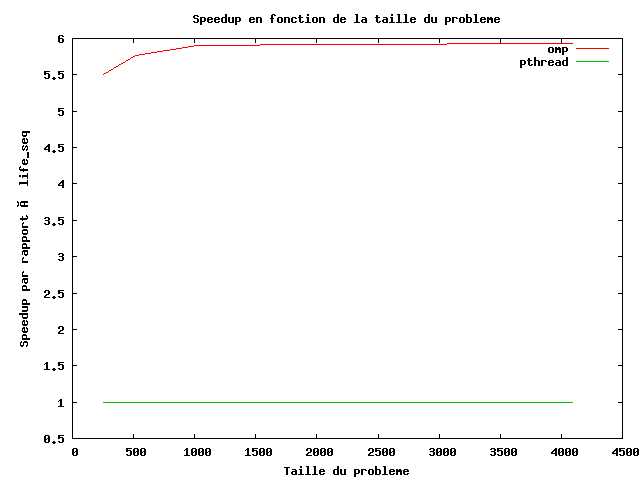
\includegraphics[scale=0.5]{single.png}
\caption{Speedups monoc\oe ur}
\label{fig:single}
\end{figure}

\newpage
\subsection{Implémentation MPI}

Le speedup de la version MPI, exécuté sur $4$ c\oe urs est une fonction constante en fonction de la taille de la grille initiale, égale environ à $4$ c'est-à-dire au nombre même de processus. Bien que ce speedup soit mesuré par rapport à la version exécutée sur $1$ c\oe ur (et non la version séquentielle), ce résultat  -- visible sur la figure \ref{fig:para} -- prouve que le jeu de la vie est extrêmement bien parallélisable puisqu'il permet d'atteindre le speed-up théoriquement maximal égal au nombre de processus mis en jeu. En ce qui concerne l'exécution sur $16$ c\oe urs, le speedup est cette fois-ci une courbe croissante (qui n'atteint qu'un speedup de $14$) en fonction de la taille de la grille. Cela peut s'expliquer par le trop grand nombre de communications induites pour la taille du problème : les calculs ne recouvrent les temps de communications qu'au fur et à mesure de l'augmentation de la taille des grilles locales au processus. Le speedup est toutefois supérieur à celui de l'exécution sur $4$ c\oe urs à partir d'une grille initiale de taille $1024$, et tend vers le maximum théorique de $16$ (il atteint $14$ pour une problème de taille $4096$ sur la figure \ref{fig:para}).

\begin{figure}[!h]
\centering
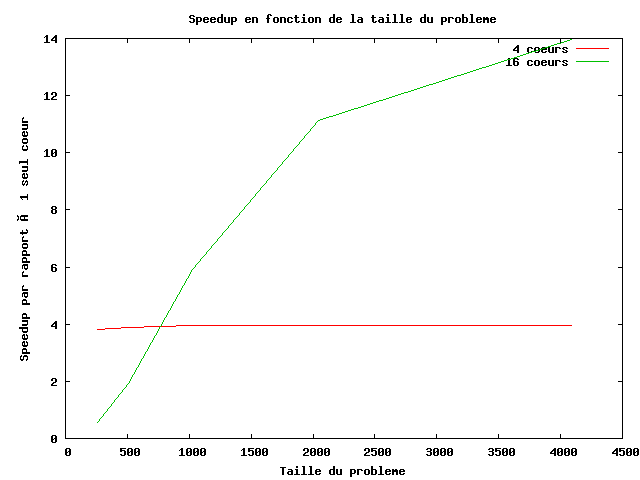
\includegraphics[scale=0.5]{para.png}
\caption{Speedups multic\oe ur}
\label{fig:para}
\end{figure}